%% ------------- Portuguese version ------------
\documentclass{sbrt}
\usepackage[english,brazil]{babel}
\usepackage[utf8]{inputenc}
\newtheorem{theorem}{Teorema}
\usepackage{comment}
\usepackage{graphicx}
\usepackage{caption}
%% ---------------------------------------------

%% If writing in English, remove the lines above
%% and uncomment the lines below

%% ------------- English version ---------------
%\documentclass[english]{sbrt}
%\usepackage[english]{babel}
%\usepackage[utf8]{inputenc}
%\newtheorem{theorem}{Theorem}
%% ---------------------------------------------

\begin{document}

\title{Comparando Containers e VMs na Hospedagem de Plataforma IoT Aberta em Edge Computing}

\author{Epaminondas A. Sousa Junior, Roberto Colistete Júnior e Moisés R. N. Ribeiro
\thanks{Epaminondas Aguiar de Sousa Junior e Moisés Renato Nunes Ribeiro, Programa de Pós-Graduação em Engenharia Elétrica, Universidade Federal do Espírito Santo, Vitória-ES, e-mail: epaminondas.sousa@aluno.ufes.br, moises@ele.ufes.br; Roberto Colistete Júnior, Departamento de Química e Física, Universidade Federal do Espírito Santo, Alegre-ES, roberto.colistete@ufes.br.}%
}

\maketitle

\markboth{XXXVIII SIMPÓSIO BRASILEIRO DE TELECOMUNICAÇÕES E PROCESSAMENTO DE SINAIS - SBrT 2020, 22--25 DE NOVEMBRO DE 2020, FLORIANÓPOLIS, SC}{} 


%% If writing in English, remove both 'resumo' and 'chave'
%% ------------- Portuguese version ------------
\begin{resumo}
A utilização de plataformas IoT tem sido amplamente utilizada para a interconexão de inúmeros dispositivos e apoio a criação de aplicações essenciais para o dia-a-dia. Esses serviços são normalmente disponibilizados em máquinas virtuais (VMs) em nuvens públicas. Todavia, a computação em borda (edge computing) em nuvens privadas está conquistado uma parcela significativa do mercado por questões de segurança, disponibilidade, latência e também custo. Outra tendência é a substituição das VMs por containers. Eles têm o potencial de implantação de plataformas IoT com alta portabilidade, escalabilidade e desempenho além de eficiência no consumo de recursos computacionais. Neste artigo, é realizada uma análise experimental de desempenho da plataforma ThingsBoard no contexto de edge computing usando VMs e containers. Sob um teste controlado, utilizamos como parâmetros o tempo médio de resposta, utilização de CPU e memória RAM e taxa de perda de pacotes, considerando diferentes cenários de carga (i.e., requisições por segundo) oriundas de dispositivos de IoT.
\end{resumo}
\begin{chave}
Plataforma IoT, edge computing, análise de desempenho.
\end{chave}

\begin{abstract}
The use of IoT platforms has been widely used for interconnecting numerous devices and supporting the creation of essential day-to-day applications. These services are typically available in virtual machines (VMs) in public clouds. However, edge computing in private clouds is gaining a significant market share for security, availability, latency and also cost reasons. Another trend is the replacement of VMs by containers. They have the potential to deploy IoT platforms with high portability, scalability and performance and efficient consumption of computing resources. In this article, an experimental performance analysis of the ThingsBoard platform is performed in the context of edge computing using VMs and containers. Under a controlled test, we use as parameters the average response time, CPU and RAM memory utilization, packet loss rate, considering different load scenarios (i.e., requests per second) from IoT devices.
\end{abstract}
\begin{keywords}
IoT platforms, edge computing, performance.
\end{keywords}



\section{Introdução}

A Internet das Coisas (IoT) é uma extensão da Internet atual que proporciona aos objetos do dia-a-dia com capacidade computacional e de comunicação, se conectarem à Internet~\cite{santos2016}. Esses objetos possuem recursos de identificação, captura de dados, processamento e de comunicação, fazendo  com que a IoT possa oferecer serviços a todos os tipos de aplicativos, garantindo ao mesmo tempo que os requisitos de segurança sejam atendidos~\cite{kurakova2013overview}. Ela está se desenvolvendo a uma velocidade surpreendente nos últimos anos, tanto que o Gartner estima que o número de dispositivos de IoT deverá ser superior a 20 bilhões, enquanto a IDC prevê que 10{\%} de todos os dados do planeta serão gerados por dispositivos de IoT já em 2020~\cite{wang2018prsfc}.

Nos últimos anos, tem surgido uma grande quantidade de plataformas IoT fazendo a interconexão dos dispositivos, ou objetos inteligentes, em sistemas que possuem diferentes número de dispositivos e objetivos. Tais plataformas se colocam como intermediárias entre as aplicações e a infraestrutura subjacente (i.e., middleware), provendo um meio padronizado para o acesso aos dados e serviços fornecidos através de uma interface de alto nível. A adoção de uma plataforma IoT pode contribuir sobremaneira para facilitar a construção de aplicações para IoT~\cite{mineraud2016gap}.

Existem muitas soluções desse tipo de middleware, que tratamos aqui como plataformas IoT, podendo ser proprietárias ou de código aberto. Várias destas são voltadas para uso específico, como é o caso de muitas plataformas proprietárias que possuem seus próprios dispositivos e mecanismos de comunicação. Essas plataformas proprietárias armazenam os dados dos dispositivos de seus clientes em nuvem privadas para processamento e backup~\cite{ganguly2016selecting}. Em relação às plataformas IoT de código aberto, estão disponíveis para o público em geral e normalmente são implementadas sobre máquinas virtuais em nuvens públicas. Algumas destas disponibilizam o seu software e/ou sua imagem pronta para instalação local, via VM e container. Estas plataformas de código aberto utilizam, normalmente, um modelo de negócio que oferece uma conta para sua utilização porém com diversas limitações que podem inclusive inviabilizar muitas das aplicações prática. Essas limitações definem, por exemplo, o número máximo de dispositivos que podem ser conectados, a taxa de transmissão, tempo de testes, capacidade e prazo de armazenamento de dados, etc.

A adoção da edge computing em IoT, por meio da instalação local das plataformas IoT de código aberto próximas aos dispositivos, possibilita as plataformas receberem um volume maior de dados, diminuição da latência, diminuição de custos, etc~\cite{qfan2018}. A instalação no contexto de edge computing dessas plataformas IoT via VMs dão flexibilidade, poder computacional e capacidade de crescimento por demanda etc. Enquanto que via container, estes são altamente portáteis, escaláveis, leves além de trazerem um ganho no tempo de implantação~\cite{santos2019avaliaccao, salah2017performance}. 

Este trabalho realiza uma análise de contexto para localizar as plataformas de IoT antes de partir para a análise experimental de desempenho de uma plataforma popular em código aberto, i.e., ThingsBoard, no contexto de edge computing, quando utilizando-a sobre VM ou container. A avaliação foca na potencial fragilidade dos containers: volume de carga de acesso oriunda de dispositivos de IoT considerando o crescimento vertiginoso do número de dispositivos. Com isso podemos avaliar de forma objetiva um dos gargalos da atual tendência da substituição das VMs por containers de forma prática em aplicações IoT. 

O restante do artigo está organizado da seguinte maneira: a Seção \ref{sec:trabfut} discute os trabalhos relacionados; na Seção \ref{sec:plat} aborda as plataformas IoT; a Seção \ref{sec:ava} apresenta a plataforma ThingsBoard na qual são feitos testes experimentais de desempenho utilizando VMs e containers e seus resultados são discutidos; por fim, na seção \ref{sec:conc} encontram-se conclusão e trabalhos futuros.

\section{Trabalhos Relacionados}
\label{sec:trabfut}

Os autores em~\cite{ganguly2016selecting} levantaram uma lista de funcionalidades e melhores práticas de uma plataforma IoT. A base de seleção é dividida em 4 fatores: oferta técnica, estratégia, presença de mercado e recomendação. O trabalho está focado na oferta técnica que está dividida em 20 itens, entre eles: open source ou pagos, protocolos suportados, SDK, aplicações mobile, gerenciamento, segurança, fóruns, entre outros. As plataformas Kaa, DeviceHive, OpenIoT e ThingSpeak são as principais de código aberto, enquanto que para trabalhos de pesquisa as plataformas comumente usadas são IoT-Framework e Lab-Of-Things. As outras plataformas são, na maioria, comerciais.

Num outro levantamento qualitativo é realizada uma avaliação em um conjunto de plataformas de IoT, tanto proprietárias como de código aberto, com o objetivo de verificar as deficiências e melhorar a integração com os ecossistemas~\cite{mineraud2016gap}. Foram analisadas 39 plataformas observando os seguintes aspectos: suporte a dispositivos heterogêneos, tipo, arquitetura, open source ou privada, possui REST, controle de acesso e serviço de descoberta. 

É apresentado em~\cite{da2018performance} um estudo de avaliação de desempenho de soluções de middleware de código aberto, com um foco maior na questão de segurança. Como abordagem para avaliação qualitativa de plataformas IoT é apresentado um conjunto de métricas para avaliação das plataformas. São identificadas 43 plataformas das quais 11 foram selecionadas para a avaliação qualitativa. Posteriormente foram classificadas 5 plataformas sendo uma proprietária e 4 open source, sendo estas: Inatel, Konker, LinkSmart, Orion+STH e SiteWhere. 

Seguindo uma linha mais quantitativa em relação à dinâmica de uso efetivo de recursos, em~\cite{ismail2018performance} é avaliado o desempenho de duas plataformas IoT open source, sendo estas: ThingsBoard e Sitewhere. O artigo avalia o desempenho e a estabilidade, utilizando os protocolos HTTP REST e MQTT, observando os seguintes parâmetros: tempo médio de resposta, vazão de dados, utilização de CPU e memória RAM e a taxa de perda de pacotes. A plataforma ThingsBoard foi instanciada com o banco de dados Cassandra, que é voltado para taxas maiores que 5 Kreq/s. As plataformas foram instanciadas em máquinas com 8GB de RAM, processador i7 de sétima geração, sendo executadas no sistema operacional Ubuntu 16.04 server.

Em termos de setup de testes, em~\cite{joy2015} é realizado  uma avaliação de desempenho entre um estudo de caso entre VMs e containers utilizando como base um software open source de gestão de conteúdo web, o Joomla. Esta aplicação é composta por dois servidores, sendo que o primeiro executa a aplicação em PHP e o segundo servidor hospeda o banco de dados. Neste artigo, de 2015, mostrou-se que o container Docker teve um melhor desempenho comparado à VM no quesito de processamento de requisições, porém elenca que as soluções utilizando containers são executadas com privilégios de root. Neste artigo, foi utilizado a ferramenta Jmeter para a geração das requisições.

Em relação à comparação direta entre VMs e containers, em~\cite{salah2017performance} é apresentado uma avaliação de desempenho de um serviço web sendo executado em container e VM. O experimento foi instanciado na nuvem da AWS, sendo que todo os recursos computacionais foram levantados na mesma região. Para a instanciação da plataforma, tanto na VM quanto em container, foram utilizados 1 vCPU e 2 GB de RAM. Para a realização dos testes, foi utilizado a ferramenta Jmeter e os testes foram executados em rajada durante apenas 20 segundos. Como resultados, a VM obteve um ganho de 125{\%} comparado com a utilização de container no quesito de tempo médio de resposta.

Finalmente focando no ambiente edge computing, os autores em~\cite{dupont2017} apresentam uma plataforma chamada Cloud4IoT para realizar a migração horizontal e vertical de funções de IoT. Para isso utilizam a edge computing em IoT para aproximar gateways para próximo dos dispositivos e podendo realizar, se necessário, a migração horizontal de funções entre gateways e vertical entre gateways e a nuvem. Utilizaram a solução de container para abrigar as funções de IoT para facilitar a migração destas, se necessário. Foram apresentados dois casos de uso, o primeiro realiza a migração horizontal de funções de IoT entre gateways para aplicação de assistência médica enquanto o segundo caso de uso explora a plataforma na migração vertical de funções IoT entre nuvem e gateways.

Os trabalhos relacionados apresentam a comparação qualitativa e quantitativa de plataformas IoT, tanto proprietárias quanto pagas; análise de desempenho entre VMs e containers; e utilização de edge computing em IoT para auxiliar soluções de assistência médica utilizando gateways implementados em container para auxiliar na implantação e migração destas. Porém, nenhum dos trabalhos citados realiza a avaliação de plataformas IoT sobre ambientes de VMs e containers, sendo este um diferencial de presente trabalho.


\section{Plataformas IoT}
\label{sec:plat}

As plataformas IoT, ou middleware, surgiram como soluções promissoras para prover a interoperabilidade e gerenciar a crescente variedade de dispositivos associados a aplicações. Essas plataformas são inseridas entre as aplicações e a infraestrutura subjacente, provendo um meio padronizado para o acesso aos dados e serviços fornecidos pelos objetos através de uma interface de alto nível. Um ponto estratégico diz respeito à adoção de plataformas IoT, ela pode contribuir para facilitar a construção de soluções de aplicações para IoT~\cite{pires2015}.

Parte das plataformas IoT existentes são construídas para cenários bem definidos, por exemplo, aplicações voltadas para a indústria que utiliza sensores com certa precisão e/ou possuem alta criticidade, enquanto a maioria das plataformas são para uso geral. As plataformas IoT, geralmente, não seguem uma arquitetura padronizada para sua criação e funcionalidades que serão disponibilizadas. 

Devido à falta de padronização na construção das plataformas IoT, para fazer comparações entre as plataformas existentes alguns autores levantam parâmetros, ou métricas, podendo ser divididos entre qualitativos e quantitativos.

As métricas qualitativas podem ser vistas como características da arquitetura e implementação da plataforma, tais como ser de código aberto ou paga, suporte a SDKs, suporte a dispositivos heterogêneos, segurança, funcionalidades oferecidas, protocolos de comunicação que são utilizados, documentação, atualizações, etc. Essas métricas não são facilmente mensuradas em números e algumas destas podem ser subjetivas, sendo observadas pelo usuário~\cite{mineraud2016gap,ganguly2016selecting}.

Muitos dos autores abordam sobre a questão de segurança dos dispositivos na conexão com a plataforma~\cite{da2018performance}. Algumas destas no momento do cadastro dos dispositivos geram um token que é inserido no cabeçalho das mensagens que os dispositivos enviam para a plataforma em que os dispositivos podem apenas fazer a publicação de dados dos sensores e/ou recebimento de dados de atuadores. Outras plataformas passam apenas um nome do dispositivo no momento de seu cadastro, e para encaminhar as informações para a plataforma necessitam de passar além do endereço da plataforma, o nome de usuário e nome cadastrado do dispositivo, podendo gerar ponto de falha.

As métricas quantitativas servem para mensurar o desempenho das plataformas. Normalmente são utilizados como parâmetros a utilização de CPU e memória RAM, vazão de dados, taxa de perda de pacotes, etc.

\section{Avaliação e Seleção para Implantação de Plataforma IoT}
\label{sec:ava}

Foram pesquisadas algumas plataformas IoT de código aberto existentes no mercado para serem adotadas para a realização dos testes de desempenho. Utilizamos alguns parâmetros qualitativos citados na Seção \ref{sec:trabfut} para a comparação das plataformas. Dentre os inúmeros parâmetros, elencamos alguns, entre eles: possui instalação local tanto em VM quanto em container, ter certo grau de popularidade no mercado e no meio acadêmico, possuir documentação fácil e por fim o suporte a múltiplos protocolos de comunicação.

Foram analisadas as seguintes plataformas: Hub-of-All-Things (H.A.T.)\footnote{https://www.hubofallthings.com}, Node-RED\footnote{https://nodered.org}, Kaa\footnote{https://www.kaaproject.org}, OpenMTC\footnote{https://www.openmtc.org}, The Things Network (TTN)\footnote{https://www.thethingsnetwork.org}, Thinger.io\footnote{https://thinger.io}, ThingsBoard\footnote{https://thingsboard.io} e ThingSpeak\footnote{https://thingspeak.com}

Das plataformas citadas acima, foi desconsiderada dos testes a plataforma Kaa, pois já fornece uma VM pronta na versão de testes e não disponibiliza a utilização local da plataforma utilizando container. As plataformas ThingerSpeak não oferece instalação local e em Thinger.io a instalação local é paga. As únicas plataformas que estão elegíveis para os testes de desempenho são a Node-RED e a ThingsBoard, porém devido à facilidade no cadastro de dispositivos e a agilidade para a montagem e realização dos testes foi escolhido a plataforma ThingsBoard. Outro fator na escolha da plataforma ThingsBoard foi o desempenho superior comparado com a plataforma SiteWhere apresentado em \cite{ismail2018performance}, utilizando o protocolo HTTP.

A plataforma ThingsBoard, escolhida para os testes, é utilizada para coleta de dados, processamento, visualização e gerenciamento de dispositivos, possuindo as seguintes características gerais:
\begin{itemize}
    \item Conectividade - suporta protocolos IoT padrão como MQTT, CoAP e HTTP;
    \item Gerenciamento de dispositivos - a plataforma dá ao usuário a capacidade de registrar, gerenciar e monitorar diferentes dispositivos. Além disso, fornece API para aplicações do lado do servidor para enviar comandos aos dispositivos e vice-versa;
    \item Armazenamento e visualização de dados - suporta bancos de dados como HSQLDB, PostgreSQL e Cassandra. A plataforma oferece dashboards personalizados aos usuários para monitorar dados em tempo real com muitos widgets configuráveis;
    \item Análise de dados - possui mecanismo de análise primária das mensagens recebidas e pode ser integrado com Kafka e Apache Spark para um processamento mais complexo.
\end{itemize}

\subsection{Cenário de avaliação}

O cenário de avaliação foi composto por dois computadores. O Computador B foi utilizado para: a) hospedar uma VM de 2 vCPU, 2 GB de RAM e Ubuntu Server 18.04 com a instalação local da plataforma ThingsBoard; e b) hospedar um container Docker com a instalação local da plataforma ThingsBoard (com a mesma configuração da VM). Foi utilizado o Virtual Box para o levantamento da VM. O Computador A foi utilizado para enviar requisições de clientes concorrentes para publicação e armazenamento de dados de dispositivos à plataforma ThingsBoard, para isso o programa Jmeter na versão 5.2.1 foi utilizado, conforme ilustrado na Figura \ref{fig:teste}.

A plataforma IoT instalada em ambos os experimentos, tanto na VM quanto no container, utilizou o banco de dados PostgreSQL e esta configuração é voltada para um número máximo de 5 Kreq/s.

Foram utilizados dois ambientes de testes, o primeiro ambiente ao qual as requisições eram geradas pelo Computador A por meio de acesso externo, realizando 11 saltos na internet pública (num cenário de edge relativamente distante), e no segundo ambiente ambos os computadores estavam em uma rede gigabit local, com todos os computadores conectados via cabo. Em cada ambiente, são realizados experimentos do Computador A para a Plataforma IoT (no Computador B) sendo implantada em container e VM. Os testes foram executados em ambiente controlado e realizados de forma isolada, para não gerar interferência no desempenho entre o modelo de implantação utilizando VM e container. Cada teste foi repetido 5 vezes e com duração de 1 minuto cada. A Tabela \ref{tab:ava_compt} apresenta as configurações dos computadores que foram usados no experimento. Nos experimentos foi testado apenas o protocolo HTTP.

\begin{table}[h]
\centering
\caption{Configuração dos computadores}
\label{tab:ava_compt}
\begin{tabular}{ccccc}
\hline
             & \textbf{Processador} & \textbf{Memória} & \textbf{Disco} & \textbf{SO} \\ \hline
 A & i7 2.6 GHz            & 16 GB DDR4           & 500 GB (SSD)         & Catalina 10.15.5                       \\ \hline
 B & i5 3 GHz              & 8 GB DDR3             & 1 TB           & Ubuntu 16.04                \\ \hline
\end{tabular}
\hspace{10mm}
\end{table}

\begin{figure}[ht]
\centering
\captionsetup{justification=centering}
\begin{center}
%\setlength{\unitlength}{0.0105in}%
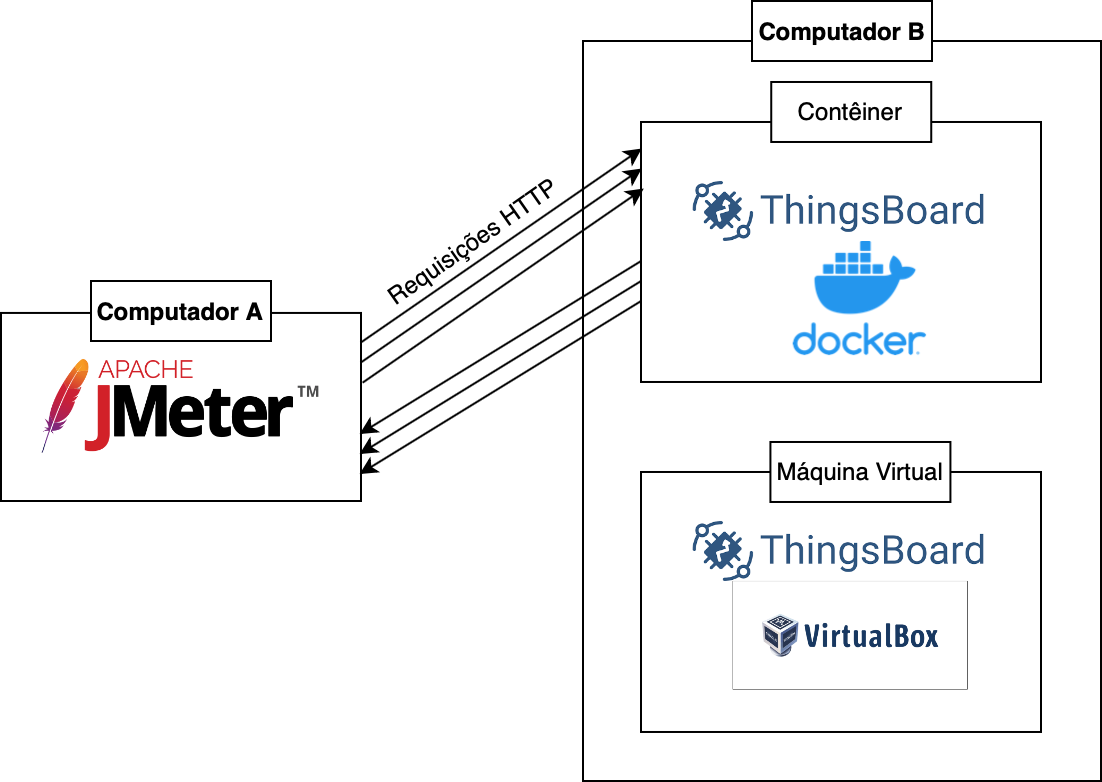
\includegraphics[scale=0.20]{sbrt2020_latex/teste.png}
\vspace*{-3mm}
\end{center}
\caption{Cenário do experimento}
\label{fig:teste}
\end{figure}

Para a avaliação de desempenho da plataforma ThingBoard nos ambientes de VM e container, os pacotes gerados para todos os testes contêm dados de 10 sensores e é variado o número de requisições de clientes concorrentes, ou mensagem por segundo (req/s) que chega à plataforma, de 1 a 1000. A ferramenta Jmeter utilizada para a geração das requisições HTTP para a plataforma IoT obtém de forma direta e simples o tempo médio de resposta das requisições, a taxa de perda de pacotes (mensagens que não foram atendidas pela plataforma proveniente da rede e/ou indisponibilidade da plataforma em atender as requisições) e vazão de dados. Para os testes com apenas 1 cliente no sistema, foram utilizados 60 amostras para calcular o tempo médio de resposta e taxa de perda de pacotes, para 1000 clientes concorrentes ou requisições foram armazenadas 60.000 amostras e para cada rodada de testes era necessário liberar espaço no disco. As informações de utilização de CPU e memória RAM foram obtidas diretamente das VMs e do Docker, dos últimos 30 segundos realizando a média de utilização das informações.

Alguns dos artigos que mostram o desempenho das plataformas IoT apresentada na Seção \ref{sec:trabfut} realizam apenas testes de rajada com duração máxima 20 segundos. Como diferencial, queremos verificar como é o desempenho da plataforma em momento de stress. Para isso, nos testes ignoramos os primeiros 30 segundos que são referentes para encher a fila de espera da plataforma IoT.

\subsection{Testes de Desempenho}
As medidas de desempenhos da plataforma ThingsBoard instalada localmente tanto em VM quanto em container utilizando acesso externo e rede local, variando o número de clientes concorrentes ou requisições que chegam à plataforma por segundo (req/s), são apresentadas nas Figuras \ref{fig:cpu_util}, \ref{fig:rtt} e \ref{fig:error}.

A Figura \ref{fig:cpu_util} apresenta o gráfico da utilização de CPU de acordo com a quantidade de requisições por segundo (req/s) que são enviados para plataforma IoT, ThingsBoard. A partir de 500 requisições por segundo, podemos observar que o container está utilizando em média 98{\%} de sua capacidade de processamento enquanto a VM utiliza 82 e 88{\%}, para acesso externo e rede local, respectivamente. A VM utiliza 100{\%} de sua capacidade de processamento a partir de 1 Kreq/s.

\begin{figure}[hbt]
\centering
\captionsetup{justification=centering}
\label{fig:cpu_util}
\begin{center}
%\setlength{\unitlength}{0.0105in}%
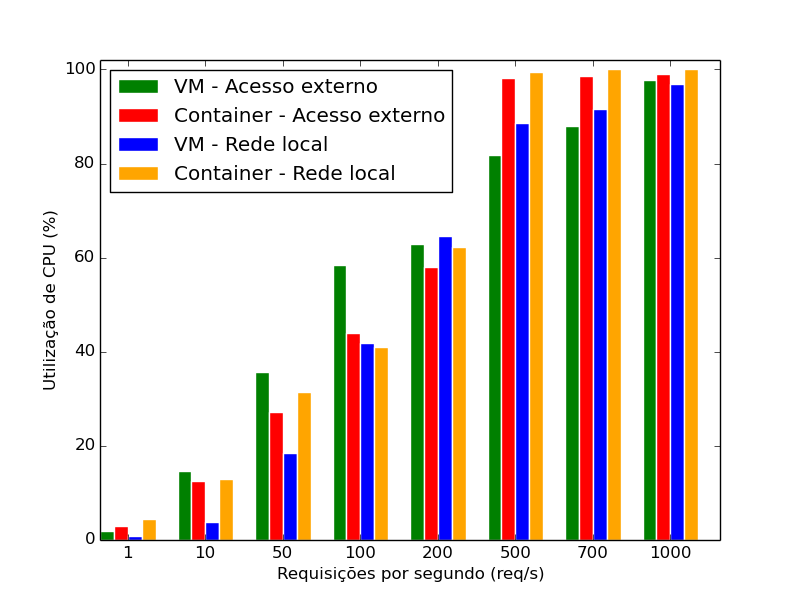
\includegraphics[scale=0.45]{sbrt2020_latex/cpu_util.png}
\vspace*{-9mm}
\end{center}
\caption{Gráfico de utilização de CPU}
\label{fig:cpu_util}
\end{figure}

É apresentado na Figura \ref{fig:rtt} o tempo médio de resposta das requisições à plataforma ThingsBoard. Podemos observar que o tempo de resposta da VM é menor comparado ao container. Quando a plataforma está recebendo 1 Kreq/s e observando os gráficos utilizando acesso externo, podemos verificar que o tempo médio de resposta da plataforma utilizando VM e container, é de 705 e 1762 ms, respectivamente, gerando uma diferença de tempo maior que 1 segundo. Em relação às VMs, o tempo médio de resposta da aplicação sendo executada na rede local é menor quanto utiliza-se acesso externo para experimentos com até 850 req/s. Para o container, o tempo médio de resposta da plataforma utilizando rede local é menor para experimentos com até 600 req/s.

\begin{figure}[h]
\centering
\captionsetup{justification=centering}
\begin{center}
%\setlength{\unitlength}{0.0105in}%
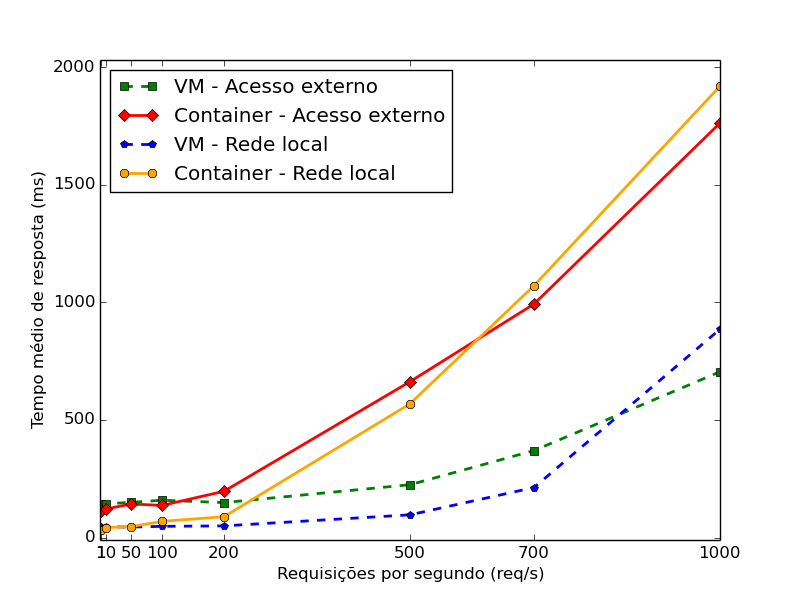
\includegraphics[scale=0.45]{sbrt2020_latex/response_time.png}
\vspace*{-9mm}
\end{center}
\caption{Tempo médio de resposta}
\label{fig:rtt}
\end{figure}

A Figura \ref{fig:error} apresenta a taxa de perda de pacotes referente à perda de pacotes na rede e/ou pacotes que foram rejeitados pela plataforma devido à fila estar cheia. A partir de 500 req/s a plataforma ThingsBoard começa a ter perda de pacotes devido à fila da aplicação estar cheia. Durante os experimentos utilizando container em rede local, a taxa de perda de pacotes foi 0{\%}. Durante os testes, especificamente, utilizando 500, 700 e 1000 req/s, começa a ter perda de pacotes, em média, depois de 30 segundos do início dos testes. Os gráficos de taxa de perda de pacotes e tempo médio de resposta possuem uma relação, pois a partir do momento que inicia a de perda dos pacotes o tempo médio de resposta é incrementado. Em \cite{da2018performance} define um limite máximo de 15{\%} tolerado pelas plataformas IoT para a taxa de perda de pacotes. Nos experimentos realizados, a taxa de perda de pacotes máxima foi de 10{\%} que é aceitável. Para um numero de req/s acima de 1000, as taxas de perda de pacotes se tornam intoleráveis. 

A utilização de memória RAM, em todos os testes realizados, foi incrementada à medida que o número de requisições por segundo aumentava, porém não passou o valor de 47{\%} de utilização. Em relação ao container, pode-se observar o crescimento gradativo da utilização de memória RAM quando incrementava o número de req/s e sua desalocação quando os testes eram interrompidos ou finalizados. Em relação às VMs, durante os testes pode-se perceber que a utilização de memória RAM se assemelhava a um gráfico crescente, ao qual a o valor era incrementado à medida que o número de req/s aumentava e quando os experimentos eram interrompidos, o valor da utilização de memória se manteve.

\begin{figure}
\centering
\captionsetup{justification=centering}
\begin{center}
%\setlength{\unitlength}{0.0105in}%
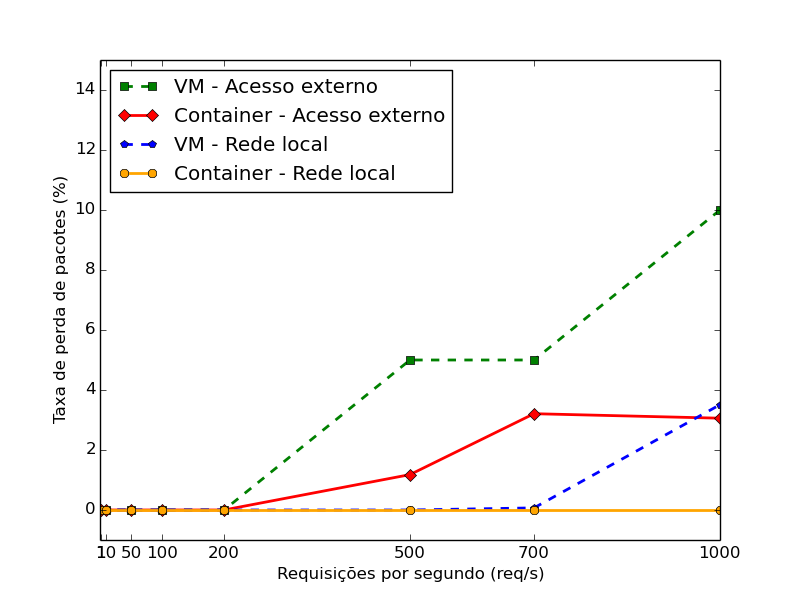
\includegraphics[scale=0.45]{sbrt2020_latex/error.png}
\vspace*{-9mm}
\end{center}
\caption{Taxa de Perda de pacotes}
\label{fig:error}
\end{figure}

\section{Conclusão}\label{sec:conc}

Neste trabalho, realizamos uma análise experimental de desempenho da plataforma ThingsBoard no centexto de edge computing, utilizando VM e container. Consideramos diferentes cenários, utilizando rede local e acesso externo e foi variado o número de requisições por segundo que chegam à plataforma, de 1 a 1000. Para os testes, a plataforma ThingsBoard foi instalada utilizando poucos recursos computacionais, com apenas 2 vCPU, 2 GB de RAM e 50 GB de Disco para armazenar os dados recebidos dos sensores. Para analisar o desempenho, utilizamos como parâmetros o tempo médio de resposta, taxa de perda de pacotes, utilização de CPU e memória RAM. 

De forma experimental, podemos observar que para aplicações de IoT, a utilização de VMs possui um melhor desempenho comparada com a utilização de container, sob os parâmetros de tempo médio de resposta e utilização de CPU. Pode-se observar também que a taxa de perda de pacotes é menor utilizando container, porém o tempo médio de resposta é maior comparado à VM. Por mais que exista a tendência da substituição das VMs por container, devido inúmeros fatores tais como portabilidade, escalabilidade, agilidade na migração e implantação de seus serviços, as VMs tiveram um ganho de desempenho de 130{\%} comparada ao container para 1 Kreq/s, sobre aplicações baseadas em IoT.

Como trabalho futuro, planejamos fazer testes utilizando: (a) ambientes de nuvem privado, tais como, OpenStack; (b) outros protocolos de comunicação, como MQTT e CoAP.


\section*{Agradecimentos}
Os autores gostariam de agradecer ao Grupo de Pesquisa NERDS, vinculado ao CNPq\footnote{dgp.cnpq.br/dgp/espelhogrupo/6925399392252343}, e pelo financiamento parcial proveniente de recursos e projetos CNPq, CAPES e FAPES.

\begin{thebibliography}{99}
\bibitem{santos2016} SANTOS, Bruno P. et al. \textit{Internet das coisas: da teoria à prática}. 
Minicursos SBRC-Simpósio Brasileiro de Redes de Computadores e Sistemas Distribuıdos, v. 31, 2016.

\bibitem{kurakova2013overview} KURAKOVA, Tatiana. \textit{Overview of the Internet of things}. 
Proceedings of the Internet of things and its enablers (INTHITEN), p. 82-94, 2013.

\bibitem{wang2018prsfc} WANG, Junxiao et al. \textit{PRSFC-IoT: A performance and resource aware orchestration system of service function chaining for Internet of Things}. 
IEEE Internet of Things Journal, v. 5, n. 3, p. 1400-1410, 2018.

\bibitem{mineraud2016gap} MINERAUD, Julien et al. \textit{A gap analysis of Internet-of-Things platforms}. 
Computer Communications, v. 89, p. 5-16, 2016.

\bibitem{ganguly2016selecting} GANGULY, Pankaj. \textit{Selecting the right IoT cloud platform}.
2016 International Conference on Internet of Things and Applications (IOTA). IEEE, p. 316-320, 2016.

\bibitem{qfan2018}Q. Fan and N. Ansari, \textit{Application Aware Workload Allocation for Edge Computing-Based IoT} 
IEEE Internet of Things Journal, vol. 5, no. 3, pp. 2146-2153, June 2018, 

\bibitem{santos2019avaliaccao} SANTOS, Brena; ENDO, Patricia Takako; SILVA, Francisco Airton. \textit{Uma Avaliação de Desempenho de Contêineres Docker Executando Diferentes SGBDs Relacionais}. 
Anais do XVIII Workshop em Desempenho de Sistemas Computacionais e de Comunicação. SBC, 2019.

\bibitem{salah2017performance} SALAH, Tasneem et al. \textit{Performance comparison between container-based and VM-based services}. 
2017 20th Conference on Innovations in Clouds, Internet and Networks (ICIN). IEEE, p. 185-190, 2017.

\bibitem{da2018performance} DA CRUZ, Mauro AA et al. \textit{Performance evaluation of IoT middleware}. 
Journal of Network and Computer Applications, v. 109, p. 53-65, 2018.

\bibitem{ismail2018performance} ISMAIL, Ahmed A.; HAMZA, Haitham S.; KOTB, Amira M. \textit{Performance evaluation of open source iot platforms} 
2018 IEEE Global Conference on Internet of Things (GCIoT). IEEE,  p. 1-5, 2018.

\bibitem{joy2015} A. M. Joy, \textit{Performance comparison between Linux containers and virtual machines}
2015 International Conference on Advances in Computer Engineering and Applications, Ghaziabad, pp. 342-346, 2015.

\bibitem{dupont2017} DUPONT, Corentin; GIAFFREDA, Raffaele; CAPRA, Luca. \textit{Edge computing in IoT context: Horizontal and vertical Linux container migration} 
2017 Global Internet of Things Summit (GIoTS). IEEE, p. 1-4, 2017.

\bibitem{pires2015} PIRES, Paulo F. et al. \textit{Plataformas para a internet das coisas} Anais do Simpósio Brasileiro de Redes de Computadores e Sistemas Distribuídos, p. 110-169, 2015.

\end{thebibliography}

%\appendix
%Aqui vão informações mais apropriadas para um apêndice.


\end{document}
